\section{针对分组密码的复杂攻击}\label{sec:4-3}

像 AES 这样被广泛使用的分组密码在被标准化之前都要经过一个漫长的选择过程,并在之后持续受到密码分析的影响。在本节中,我们将调查多年来开发的一些攻击技术。

在 \ref{subsec:4-3-1} 小节,我们将讨论针对密码设计的攻击,这些攻击可能会从对明文/密文对的观察中获得关于密钥的信息。与暴力穷举搜索攻击不同,这些\textbf{算法攻击(algorithmic attack)}依赖于对特定分组密码内部结构的巧妙分析。

在 \ref{subsec:4-3-2} 小节,我们将介绍一种非常不同的攻击类别,称为\textbf{边信道攻击(side-channel attack)}。在分析任何密码系统时,我们都会考虑对手与密码系统的用户交互的情况。在这些交互的过程中,对手收集到的信息可能会帮助其破解系统。在本书中,我们通常假设这种信息仅限于用户的输入/输出行为(例如明文/密文对)。然而,这个假设忽略了一个事实,即\textbf{计算本身是一个物理过程}。正如我们将看到的,在一些情况下,对手有可能通过测量计算的某些物理特性,例如运行时间或功耗,来破解一个密码系统。

另一类针对密码系统的物理实现的攻击是\textbf{错误注入攻击(fault-injection attack)},我们将在 \ref{subsec:4-3-3} 小节讨论。最后,在 \ref{subsec:4-3-4} 小节,我们还会考虑另一类算法攻击,即对手可以利用\textbf{量子力学}定律来加快其计算速度。

这些巧妙的攻击导出了两个非常重要的观点:
\begin{enumerate}
	\item 密码学的普通用户应该只使用像 AES 这样的标准化算法,而不是去设计他们自己的分组密码。
	\item 最好不要自己去实现算法,因为自己的实现很可能容易受到边信道攻击。最好是使用已经被广泛验证的成熟密码库。
\end{enumerate}
为了进一步强调这些观点,我们鼓励任何第一次了解 AES 内部工作原理的人作出以下娱乐性的承诺,它最早由 Jeff Moser 提出:
\begin{quote}
我保证,一旦我看到AES到底有多简单,我就\emph{不会}在生产代码中去实现它,就算它真的很有趣。这个承诺将一直有效,直到我了解了所有关于边信道攻击及其反制对策的知识,以至于我对自己实现AES失去兴趣。
\end{quote}

\subsection{算法攻击}\label{subsec:4-3-1}

攻击分组密码的设计是一个庞大的领域,其中包含许多复杂的技术:线性密码分析、差分密码分析、滑动攻击、飞去来器攻击等等。我们参考了 \cite{standaert2003cryptanalysis},这篇论文对很多已有的优雅攻击方案进行了详细的调研。在此,我们简要介绍一种称为\emph{线性密码分析}的技术,该技术已被成功用于破解 DES 密码。这种技术由日本密码学家松井充 (Mitsuru Matsui) 提出,它解释了这个问题,即为什么我们一直说设计有效的密码是非常具有挑战性的一项工作 \cite{matsui1993linear,matsui1994first}。另外,这种方法已经被证明对 AES 不起作用。

\begin{snote}[线性密码分析。]
令 $(E,D)$ 是一个数据分组和密钥都是比特序列的分组密码,即 $\mathcal{M}=\mathcal{C}=\{0,1\}^n$,$\mathcal{K}=\{0,1\}^h$。

对于一个比特序列 $m\in\{0,1\}^n$ 和一个比特位置集合 $S\subseteq\{0,\dots,n-1\}$,我们用 $m[S]$ 表示 $S$ 中对应位置的比特的异或。也就是说,如果 $S=\{i_1,\dots,i_\ell\}$,则 $m[S]:=m[i_1]\oplus\dots\oplus m[i_\ell]$。

如果存在比特位置集合 $S_0,S_1\subseteq\{0,\dots,n-1\}$ 和 $S_2\subseteq\{0,\dots,h-1\}$,使得对于\emph{所有的}密钥 $k\in\mathcal{K}$ 和\emph{随机选出的} $m\in\mathcal{M}$,都有:
\begin{equation}\label{eq:4-14}
\Pr
\Bigm[
m[S_0]\oplus E(k,m)[S_1]=k[S_2]
\Bigm]
\geq
\frac{1}{2}+\epsilon
\end{equation}
我们就称分组密码 $(E,D)$ 包含一个\textbf{线性关系 (linear relation)}。其中的 $\epsilon$ 是一个不可忽略不计的值,称为\textbf{偏差 (bias)}。对于一个``理想的"密码,明文和密文表现地就像两个相互独立的序列一样,所以式 \ref{eq:4-14} 中的关系 $m[S_0]\oplus E(k,m)[S_1]=k[S_2]$ 恰好以 $1/2$ 的概率成立,因此有 $\epsilon=0$。令人惊讶的是,DES 密码就有一个线性关系,其偏差 $\epsilon$ 虽小但不可忽略不计。

让我们看看线性关系是如何招致攻击的。考虑一个密码 $(E,D)$,它有一个如式 \ref{eq:4-14} 那样的线性关系,对于某个不可忽略不计的 $\epsilon>0$ 成立。我们假设线性关系是明确的,所以攻击者知道关系中使用的集合 $S_0$,$S_1$ 和 $S_2$。假设对于某个未知的密钥 $k\in\mathcal{K}$,攻击者能够获得许多明文/密文对 $(m_i,c_i)$,$i=1,\dots,t$。我们假设消息 $m_1,\dots,m_t$ 是从 $\mathcal{M}$ 中独立均匀采样的,并且 $c_i=E(k,m_i)$ 对于 $i=1,\dots,t$ 成立。利用这些信息,假设攻击者得到了足够多的明文/密文对,它就可以了解关于密钥 $k$ 的一个比特的信息,即 $k[S_2]\in\{0,1\}$。下面的定理说明了这一点。
\end{snote}

\begin{lemma}\label{lemma:4-3}
假设 $(E, D)$ 是一个满足式 \ref{eq:4-14} 的分组密码。令 $m_1,\dots,m_t$ 是从消息空间 $\mathcal{M}$ 中均匀独立采样得到的消息,令 $c_i:=E(k,m_i)$ 对 $i=1,\dots,t$ 成立。那么:
\begin{equation}\label{eq:4-15}
\Pr
\Bigm[
k[S_2]={\rm Majority}^t_{i=1}(m_i[S_0]\oplus c_i[S_1])
\Bigm]
\geq1-e^{-{t\epsilon^2}/{2}}
\end{equation}
\end{lemma}

这里,$\rm Majority$ 表示对给定的比特进行多数投票;例如,对于输入 $(0,0,1)$,$\rm Majority$ 的结果就是 $0$;对于 $(0,1,1)$,结果就是 $1$。直接应用经典切尔诺夫约束(Chernoff bound)就可以证明该引理。

式 \ref{eq:4-15} 中的下界表明,一旦给定的明文/密文对的数量超过 ${4}/{\epsilon^2}$,$\rm Majority$ 的输出等于 $k[S_2]$ 的概率就会超过 $86\%$。这样,攻击者就可以从给定的明文/密文对中计算出 $k[S_2]$,并获得关于密钥的一个比特的信息。虽然仅一比特的信息看起来可能不多,但它是迈向更强攻击的垫脚石,而后者可能就能暴露整个密钥。

\begin{snote}[对 DES 的线性密码分析。]
松井充表明,DES 密码中的 $14$ 轮加密中存在一个线性关系,其中的偏差至少有 $\epsilon\geq2^{-21}$。事实上,我们可以得到两个线性关系:其中一个利用 DES 加密电路的线性性质,另一个则利用解密电路的线性性质。对于一个 $64$ 比特的明文 $m$,令 $m_{\rm L}$ 和 $m_{\rm R}$ 分别表示 $m$ 的左 $32$ 比特和右 $32$ 比特。同样地,对于一个 $64$ 比特的密文 $c$,令 $c_{\rm L}$ 和 $c_{\rm R}$ 分别表示 $c$ 的左 $32$ 比特和右 $32$ 比特。那么 DES 的中包含的两个线性关系是:
\begin{equation}\label{eq:4-16}
	\begin{aligned}
		m_{\rm R}[17,18,24]\oplus c_{\rm L}[7,18,24,29]\oplus c_{\rm R}[15] & = k[S_{\rm e}]\\
		c_{\rm R}[17,18,24]\oplus m_{\rm L}[7,18,24,29]\oplus m_{\rm R}[15] & = k[S_{\rm d}]
	\end{aligned}
\end{equation}
其中 $S_{\rm e},S_{\rm d}\subseteq\{0,\dots,55\}$ 是 $56$ 比特密钥 $k$ 的某两个比特位置集合。当应用到 $14$ 轮 DES 中时,上面两个关系都有偏差 $\epsilon\geq2^{-21}$。

通过将 DES 的首轮和末轮(即第 $1$ 轮和第 $16$ 轮)纳入它们,这两个关系就可以被扩展到全部 $16$ 轮 DES 中。令 $k_1$ 是第一轮密钥,$k_{16}$ 是最后一轮密钥。根据 DES 轮函数的定义,我们从式 \ref{eq:4-16} 可以得到全部 $16$ 轮 DES 电路的以下关系:
\begin{align}
\Big(m_{\rm L}\oplus F(k_1,m_{\rm R})\Big)[17,18,24]\oplus c_{\rm R}[7,18,24,29]\oplus\Big(c_{\rm L}\oplus F(k_{16},c_{\rm R})\Big)[15]=k[S_{\rm e}'] \label{eq:4-17}\\
\Big(c_{\rm L}\oplus F(k_{16},c_{\rm R})\Big)[17,18,24]\oplus m_{\rm R}[7,18,24,29]\oplus\Big(m_{\rm L}\oplus F(k_1,m_{\rm R})\Big)[15]=k[S_{\rm d}'] \label{eq:4-18}
\end{align}
其中 $S_{\rm e}',S_{\rm d}'\subseteq\{0,\dots,55\}$ 是 $56$ 比特密钥 $k$ 中的两个适当的比特位置集合。

我们首先考察式 \ref{eq:4-17} 中的关系。$F(k_1,m_{\rm R})$ 的第 $17,18,24$ 比特是同一个的 S 盒的结果,因此它们只取决于 $k_1$ 的 $6$ 个比特。类似地,$F(k_{16},c_{\rm R})[15]$ 只取决于 $k_{16}$ 的 $6$ 个比特。因此,式 \ref{eq:4-17} 的左手边只取决于密钥 $k$ 的 $12$ 比特,我们用 $k^{(12)}$ 表示这 $12$ 个比特。我们知道,当这 $12$ 比特被设定为正确的值时,式 \ref{eq:4-17} 的左手边在计算随机的明文/密文对时相对于 $k[S_{\rm e}']$ 表现出约 $2^{-21}$ 的偏差。而当这 $12$ 比特被设定为错误的值时,式 \ref{eq:4-17} 中的偏差就小得多。正如我们将要看到的,这个结论已经在实验中得到了验证。

这一观察让攻击者能以下面介绍的方式恢复密钥 $k$ 的 $12$ 比特 $k^{(12)}$。给定一个由 $t$ 个明文/密文对组成的列表 $L$(例如 $t=2^{43}$),攻击者进行以下操作:
\begin{itemize}
    \item 步骤 $1$:对于密钥比特 $k^{(12)}$ 的 $2^{12}$ 种候选情况中的每一个,计算式 \ref{eq:4-17} 中的偏差。也就是说,对 $L$ 中的所有 $t$ 个明文/密文对计算式 \ref{eq:4-17} 的左手边,令 $t_0$ 为表达式结果为 $0$ 的次数。偏差的计算方法是$\epsilon=|(t_0/t)-(1/2)|$。这就产生了一个由 $2^{12}$ 个偏差组成的向量,每一个 $k^{(12)}$ 的 $12$ 比特候选值都对应着一个偏差。
	\item 步骤 $2$:将 $2^{12}$ 个候选值按其偏差从大到小排序。如果给定的明文/密文对的列表 $L$ 足够大,那么偏差最高的 $12$ 位候选值就最有可能等于 $k^{(12)}$,这样就可以恢复密钥中的 $12$ 比特。一旦知道了 $k^{(12)}$,我们就可以用引理 \ref{lemma:4-3} 确定 $k[S_{\rm e}']$ 这个比特,从而得到密钥 $k$ 中共计 $13$ 个比特。
\end{itemize}
攻击者可以用完全相同的方法由式 \ref{eq:4-18} 得到 $k$ 的另外 $13$ 个比特,这样就一共得到了 $26$ 比特。剩余的 $56-26=30$ 个比特就可以通过暴力穷举搜索来恢复。

单纯地计算步骤 $1$ 中的偏差需要耗时 $2^{12}\times t$:对于每个 $k^{(12)}$ 的候选值,我们必须在 $L$ 中的所有 $t$ 个明文/密文对上计算式 \ref{eq:4-17}。但下面的思路能将工作时间减少到大约 $t$。对于一个给定的数对 $(m,c)$,式 \ref{eq:4-17} 的左手边只需 $(m,c)$ 中的 $13$ 个比特就能计算出来:计算 $F(k_1,m_{\rm R})[17,18,24]$ 需要 $m$ 的 $6$ 个比特,计算 $F(k_{16},c_{\rm R})[15]$ 需要 $c$ 的 $6$ 个比特,最后还需要 $m_{\rm L}[17,18,24]\oplus c_{\rm R}[7,18,24,29]\oplus c_{\rm L}[15]$ 这 $1$ 个比特。这 $13$ 个比特足以对任何候选密钥计算式 \ref{eq:4-17} 的左手边。两个在这 $13$ 比特上达成一致的明文/密文对将总是导出式 \ref{eq:4-17} 中的相同值。我们把这 $13$ 个比特称为明文/密文对的\emph{类型(type)}。

在计算步骤 $1$ 中的偏差之前,我们需要建立一个大小为 $2^{13}$ 的表,用来计算 $L$ 中每种类型的明文/密文对的数量。对于 $b\in\{0,1\}^{13}$,表项 $b$ 是类型为 $b$ 的明文/密文对的数量。构建这张表需要耗时 $t$,但一旦构建了这张表,计算步骤 $1$ 中的所有偏差可以在 $2^{12}\times 2^{13}=2^{25}$ 的时间内完成,这远远小于 $t$。因此,步骤 $1$ 中的主要工作其实是计算每种类型的明文/密文对的数量。

松井充表明,给定一个包含 $2^{43}$ 项明文/密文对的列表,这种攻击成功的概率为 $85\%$,需要约 $2^{43}$ 次 DES 电路的计算。Junod 的实验结果表明,在 $2^{43}$ 个明文/密文对中,步骤 $1$ 中的前 $2700$ 个最有可能的候选值中就有很大概率包含密钥正确的 $26$ 比特 \cite{junod2001complexity}。换句话说,为了恢复全部 $56$ 比特的密钥,对剩余 $30$ 比特的穷举搜索平均只需进行 $2700\approx 2^{11.4}$ 次。总的来说,攻击 DES 耗时的主要部分是对 DES 电路进行平均大约 $2^{30}\times 2^{11.4}=2^{41.4}$ 次的评估 \cite{junod2001complexity}。
\end{snote}

\begin{snote}[教训。]
针对 DES 的线性密码分析之所以能够实现,是因为它的第五个 $S$ 盒 $S_5$ 恰好能在某种程度上被一个线性函数逼近。$S_5$ 的线性性质导致 DES 密码中包含线性关系,而它可以被利用来恢复秘钥。这种攻击只需 $2^{41}$ 次 DES 运算,远远少于穷举搜索所需的 $2^{56}$ 次。然而,与穷举搜索不同,这种攻击需要大量的明文/密文对:所需的 $2^{43}$ 对明文数据相当于 $64$ \emph{兆字节}。尽管如此,这还是说明了设计安全的分组密码是多么困难,以及为什么应该只使用标准化的和经过充分论证的密码。

多年来,线性密码分析已被推广到允许在明文、密文和密钥比特之间存在更复杂的非线性关系。这些推广之后被用来对付其他的分组密码,如 LOKI91 和 Q。
\end{snote}

\subsection{边信道攻击}\label{subsec:4-3-2}

边信道攻击的攻击对象并不是作为数学对象的密码系统。相反,它们利用的是其物理实现中不经意间泄露的信息。

考察一个攻击者,它在观察密码系统对机密数据的操作,比如对密钥的操作。攻击者可以获取比系统的输入/输出行为多得多的信息。两个重要的例子是:
\begin{itemize}
	\item \textbf{时间边信道}:在一个易受攻击的实现中,加密一个明文分组所需的时间可能取决于密钥的值。因此,通过测量加密的时间,攻击者就能获取关于密钥的信息。
	\item \textbf{功耗边信道}:在一个易受攻击的实现中,硬件在加密一个明文分组时使用的电量可能取决于密钥的值。想从智能卡等设备中提取密钥,攻击者可以在设备运行时测量其功耗情况,从而了解密钥的相关信息。
\end{itemize}
许多其他的边信道也被用来实现攻击,比如设备在加密时发出的电磁辐射、热量 \cite{murdoch2006hot} 乃至声音 \cite{genkin2014rsa}。

\subsubsection{计时攻击}

计时攻击是对密码学实现的一个重大威胁。远程网络攻击者可以测量计时信息,它可以与受害者服务器交互,并测算服务器对特定请求的响应时间。对于一个存在漏洞的实现,其响应时间就可以透露密钥的信息。与受害者同在一台本地设备工作的攻击者也同样能获得计时信息,比如一个低权限的进程可能会以这种方式从高权限的进程中提取密钥。在这种情况下,攻击者可以对其目标进行非常精确的时间测量。本地的和远程的计时攻击都已经被充分地研究与展示了。

在本小节中,我们会介绍针对 AES 的计时攻击,该攻击利用了受害者设备上的内存缓存行为。我们假设对手可以准确地测算受害者的运行时间,因为它可以请求受害者用 AES 加密一个明文分组。我们提出的攻击利用了机器分层存储结构中的缓存设计所导致的时间变化现象。

现代处理器使用分层的缓存结构来加快对内存的访问速度。缓存中速度最快的一层称为 L1 缓存,它的容量最小(比如$64$ KB)。数据以 $64$ 字节分组的形式(称为缓存行)被加载到 L1 缓存中。注意,将一行数据加载到 L1 缓存中比读取已在缓存中的一行耗时更多。

这种缓存引起的时间差异导致了基于快速查找表的 AES 实现很容易受到密钥恢复攻击,而忽略这种缓存效应的 AES 实现会受到毁灭性的打击。

回顾一下基于查找表的 AES 实现。除了最后一轮,其他轮都使用了四张表 $T_0,T_1,T_2,T_3$。由于最后一轮不包括 $\mathtt{MixColumns}$ 运算,所以这一轮的计算使用另一张 $S$ 表。假设当 AES 的每次执行开始时,$S$ 表尚不在 L1 缓存中,那么在第一次读取表项时,表的其中一部分就会被加载到 L1 缓存中。因此,第一次的读取会很慢,但随后对同一条目的读取会快很多,因为数据已经被缓存了。由于 $S$ 表只在 AES 的最后一轮使用,所以在最后一轮之前,$S$ 表中的任何部分都不会被加载到缓存中。

令 $A=(a_i)_{i=0,\dots,15}$ 表示最后一轮的 $4\times4$ 输入,令 $(w_i)_{i=0,...,15}$ 表示最后一轮的 $4\times4$ 密钥,那么 AES 的最终输出可以表示为以下的 $4\times4$ 矩阵:
\begin{equation}\label{eq:4-19}
	C=(c_{i,j})=
	\begin{pmatrix}
		S[a_0]+w_0 & S[a_1]+w_1 & S[a_2]+w_2 & S[a_3]+w_3\\
		S[a_5]+w_4 & S[a_6]+w_5 & S[a_7]+w_6 & S[a_4]+w_7\\
		S[a_{10}]+w_8 & S[a_{11}]+w_9 & S[a_8]+w_{10} & S[a_9]+w_{11}\\
		S[a_{15}]+w_{12} & S[a_{12}]+w_{13} & S[a_{13}]+w_{14} & S[a_{14}]+w_{15}
	\end{pmatrix}
\end{equation}
攻击者能够得到这个最终输出的 $C$。

为了实施攻击,考虑输出矩阵 $C$ 中的两个连续项,例如 $c_0=S[a_0]+w_0$ 和 $c_1=S[a_1]+w_1$。将两项相减,我们可以发现,当 $a_0=a_1$ 时,有以下关系成立:
\[
c_0-c_1=w_0-w_1
\]
因此,在令 $\Delta:=w_0-w_1$ 的情况下,只要有 $a_0=a_1$,就有 $c_0-c_1=\Delta$ 成立。此外,当 $a_0\neq a_1$ 时,$S$ 表的结构能确保 $c_0-c_1\neq\Delta$。

这里的关键点是,只要 $a_0=a_1$,读取 $S[a_0]$ 时就会把 $S$ 的 $a_0$ 项加载到 L1 缓存中,这样 $S[a_1]$ 对这一项的第二次访问就会快很多。然而,如果 $a_0\neq a_1$,有可能两次读取时缓存都不会命中,这样两次都会很慢。因此,当 $a_0=a_1$ 时,整个 AES 密码的预期运行时间要比 $a_0\neq a_1$ 时略少。

攻击者现在的计划就是在许多随机的输入分组上运行受害者的 AES 实现,并测量其运行时间。对于每个 $\Delta\in\{0,1\}^8$,攻击者创建一张表 $L_\Delta$,其中包含所有满足 $c_0-c_1=\Delta$ 的输出密文。随后,对于每个 $\Delta$,攻击者考察计算 $L_\Delta$ 中所有密文的平均时间。只要样本足够多,对于满足 $\Delta=w_0-w_1$ 的 $\Delta$ 值,攻击者必然可以得到最低的平均运行时间。因此,计时信息就揭示了关于最后一轮密钥的一个线性关系:$w_0-w_1=\Delta$。

假设 AES 实现以某种顺序计算式 \ref{eq:4-19} 中的各项。对 $C$ 中的不同连续项 $c_i$ 和 $c_{i+1}$ 重复上述计时过程,可以发现最后一轮密钥的每两个连续字节之间都存在 ${\rm GF}(2^8)$ 上的差异。那么,如果最后一轮密钥的第一个字节是已知的,那么最后一轮密钥的所有剩余字节都可以从已知的差异中计算出来。此外,由于 AES-128 的密钥扩展是可逆的,因此从最后一轮密钥中重建 AES-128 的密钥是一件很简单的事情。

为了完成攻击,攻击者只需尝试最后一个轮密钥的第一个字节的所有 $256$ 个可能值。对于每个候选值,攻击者都会得到一个可能的 AES-128 密钥。攻击者可以把这个密钥用在一些已知的明文/密文对上,以此来验证它的正确性。一旦找到一个正确的 AES-128 密钥,攻击者就获得了所需的密钥。

这种攻击是由 Joseph Bonneau 和 Ilya Mironov 提出的,它在实践中效果相当好 \cite{bonneau2006cache}。他们在 Pentium IV Xeon 上的实验对大约 $2^{20}$ 次加密算法进行计时测算,成功地恢复了一个 AES 密钥。该攻击只需要几分钟的时间就能完成。我们注意到,Pentium IV Xeon 使用的是 $32$ 字节的高速缓存总线,因此 $S$ 表会被分成八行。

\begin{snote}[缓和措施。]
抵抗针对 AES 的计时攻击的最简单方法是使用 AES-NI 指令在硬件中实现 AES。这些指令比软件实现的速度更快,并且不管密钥和输入分组怎么变化,加解密所需要的时间总是相同的。

在没有内置 AES 指令的处理器上,我们不得不使用 AES 的软件实现。防范高速缓存计时攻击的一个方法是使用 AES 的无表实现。有几种这样的 AES 实现,它们使用一种叫做\textbf{比特切割 (bit-slicing)} 的技术,在软件中提供合理的性能,并且可以抵抗计时攻击。

另一种方法是在每次调用 AES 之前将表 $T_0,T_1,T_2,T_3$ 和 $S$ 都预先加载到 L1 缓存中,这可以防止基于缓存的计时攻击。但前提是,当 AES 执行时,必须确保这些表不会被从 L1 缓存中清除出去。而确保这些表能按照设想留在 L1 缓存中,在现代处理器上是不容易的。因为中断可能会在 AES 执行过程中把缓存行清除出高速缓存,而\emph{超线程}技术也允许多个线程同时运行在同一个物理内核上,当一个线程把 AES 表加载到 L1 缓存中后,另一个线程所执行的其他程序也可能在无意中将其清除。

还有一种方法是将 AES 的执行时间拉到最大来防止计时攻击,但这显然对性能影响很大。

最后,我们要强调的是,简单地在每次 AES 执行后添加随机数量的无效指令来填充运行时间并不能防止计时攻击,因为只要攻击者获得更多样本,它就可以通过计算平均值将这些无效的扰动清除出去。
\end{snote}

\subsubsection{针对 AES 实现的功耗攻击}

一个设备在运行过程中所消耗的电量也可以泄露设备内部工作的信息,包括存储在设备上的密钥。让我们看看攻击者如何利用功耗测量来快速提取物理设备上的密钥。

作为一个例子,考察一种带有嵌入式芯片的信用卡,该芯片中包含一个 AES 密钥。为了进行购买,用户将信用卡插入一个销售终端设备。终端机向信用卡提供交易细节,而信用卡则使用内嵌的 AES 密钥来授权该交易。我们还会在之后的章节中更详细地讨论这个过程。

由于嵌入式芯片必须从终端获取电源(它是无源的),因此终端很容易测量芯片在特定时间间隔内的功耗。特别地,攻击者可以在运行 AES 算法时测量所消耗的电量。图 \ref{fig:4-12-a} 展示了一个测试设备在四次运行 AES-128 算法时的耗电量($x$轴是时间,$y$轴是功率),其中每个驼峰就代表 AES 的一次运行,而每个驼峰中的十个尖峰就代表着 AES-128 中的十轮计算。

\begin{snote}[简单功耗分析。]
假设某种密码实现中包含了一个分支指令,它取决于密钥中的一个比特。比如说,当密钥的最小有效比特 (least significant bit, LSB) 为 $1$ 时就执行该分支,否则就不执行该分支。由于执行分支比不执行分支要消耗更多的电量,所以当该比特为 $1$ 时,功耗轨迹图会在该点处显示一个尖峰,否则就没有尖峰。攻击者可以简单地在功耗轨迹图的适当位置寻找一个尖峰,以此来了解关键比特的情况。通过考察多个依赖密钥中特定比特的分支指令,攻击者就能够恢复出密钥的大部分信息。这种攻击方式对某些密码系统的简单实现非常有效(比如 RSA,我们将在之后的章节中介绍)。

上一段所介绍的攻击方式称为\textbf{简单功耗分析 (simple power analysis, SPA)},它对 AES 并不起作用,因为在加密过程中,AES 轮密钥会被简单地异或到密码状态中。而异或指令所消耗的功率只在很小程度上取决于其操作数,因此无法透露关于密钥的有用信息。因此 AES 能够抵抗这种简单功耗分析,这也是它的一个重要优点。
\end{snote}

\begin{figure}
  \centering
  \subfigure[四次迭代 AES 的功耗]{
  	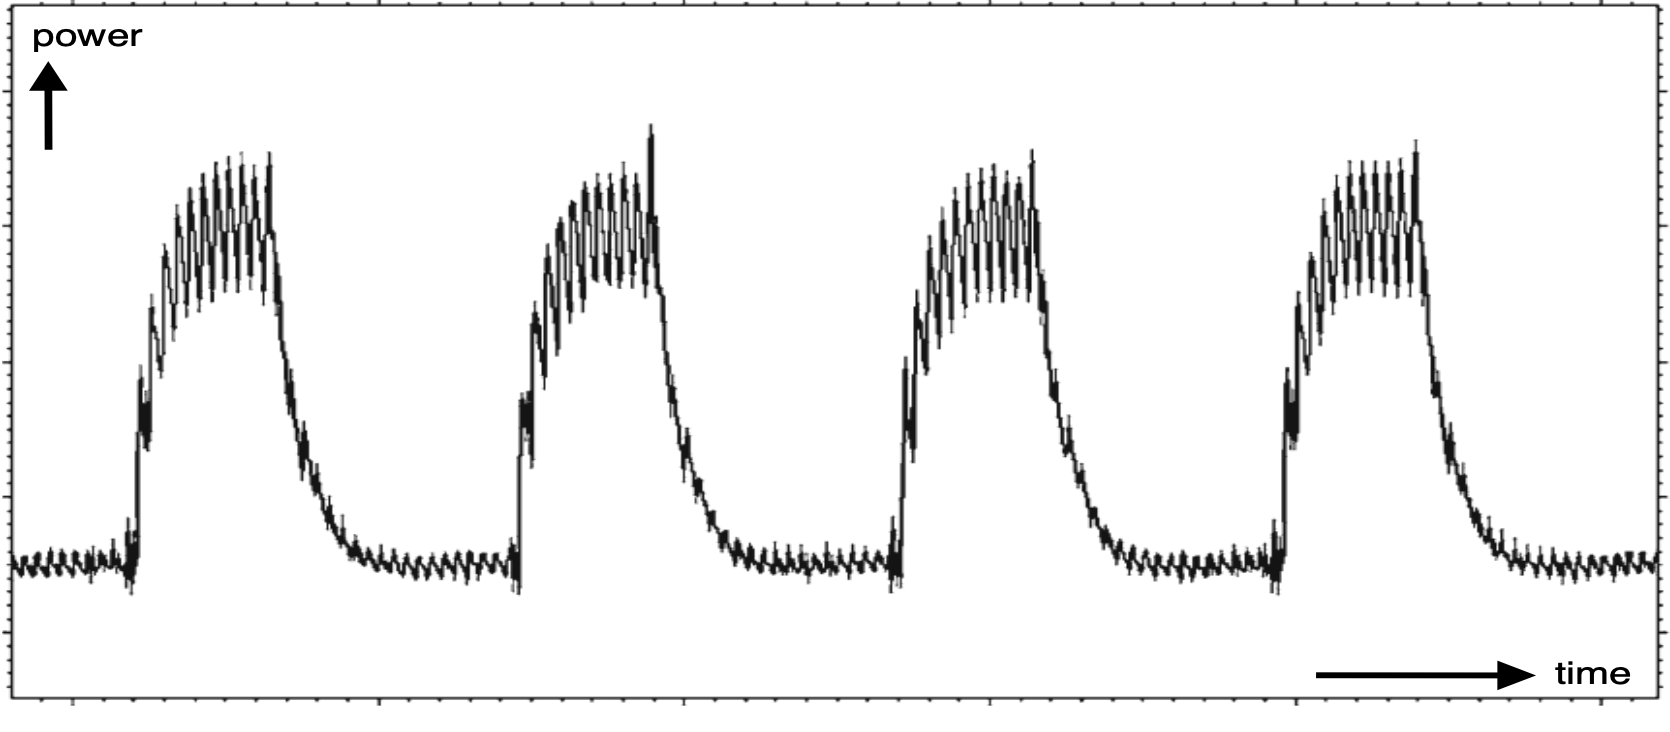
\includegraphics[width=0.4\linewidth]{figures/chapter4/fig12-a.png}
  	\label{fig:4-12-a}
  }
  \quad\quad\quad
  \subfigure[S盒LSB的输出为$0$和为$1$的情况]{
  	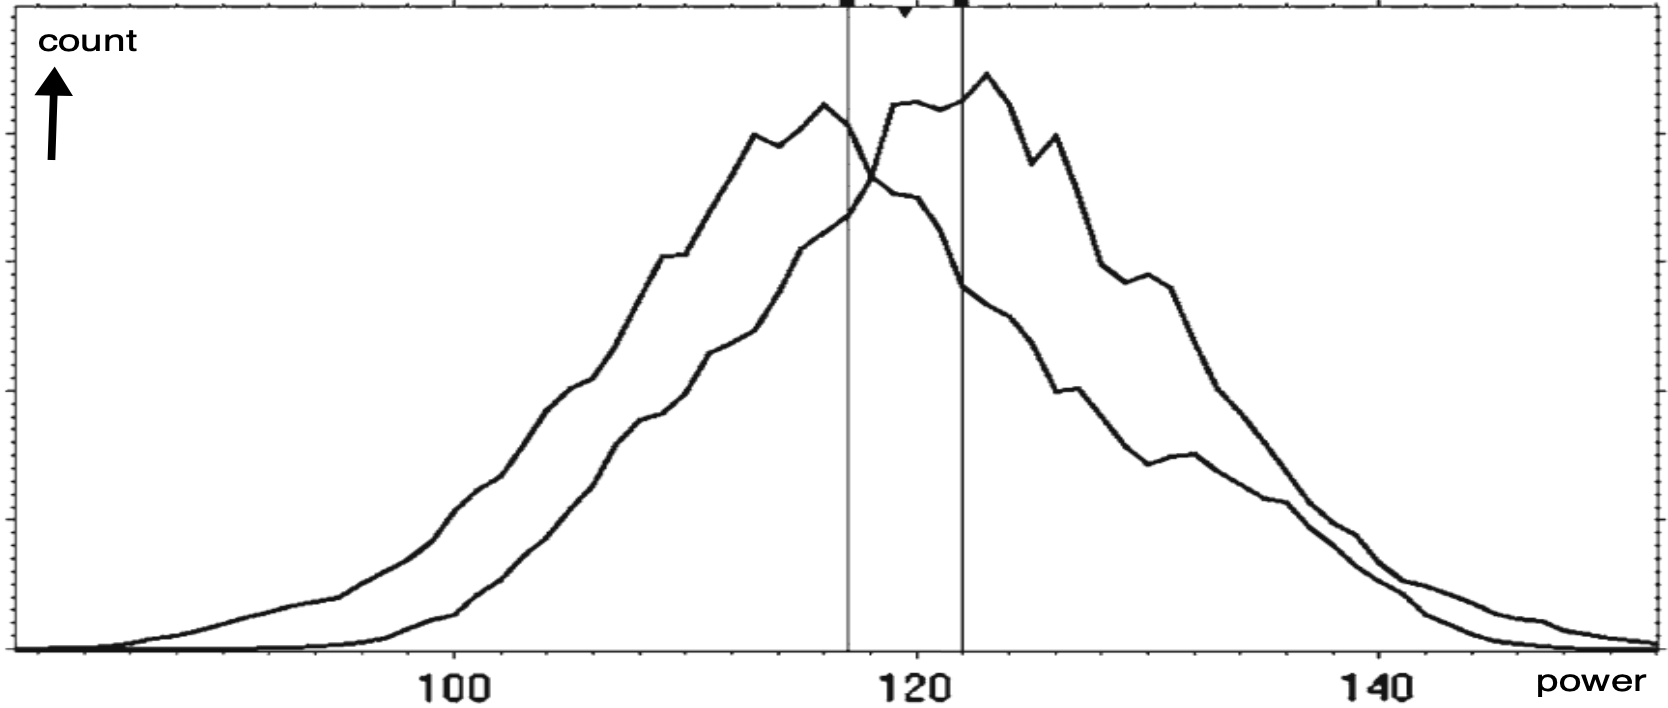
\includegraphics[width=0.4\linewidth]{figures/chapter4/fig12-b.png}
  	\label{fig:4-12-b}
  }
  
  \subfigure[功耗差分]{
  	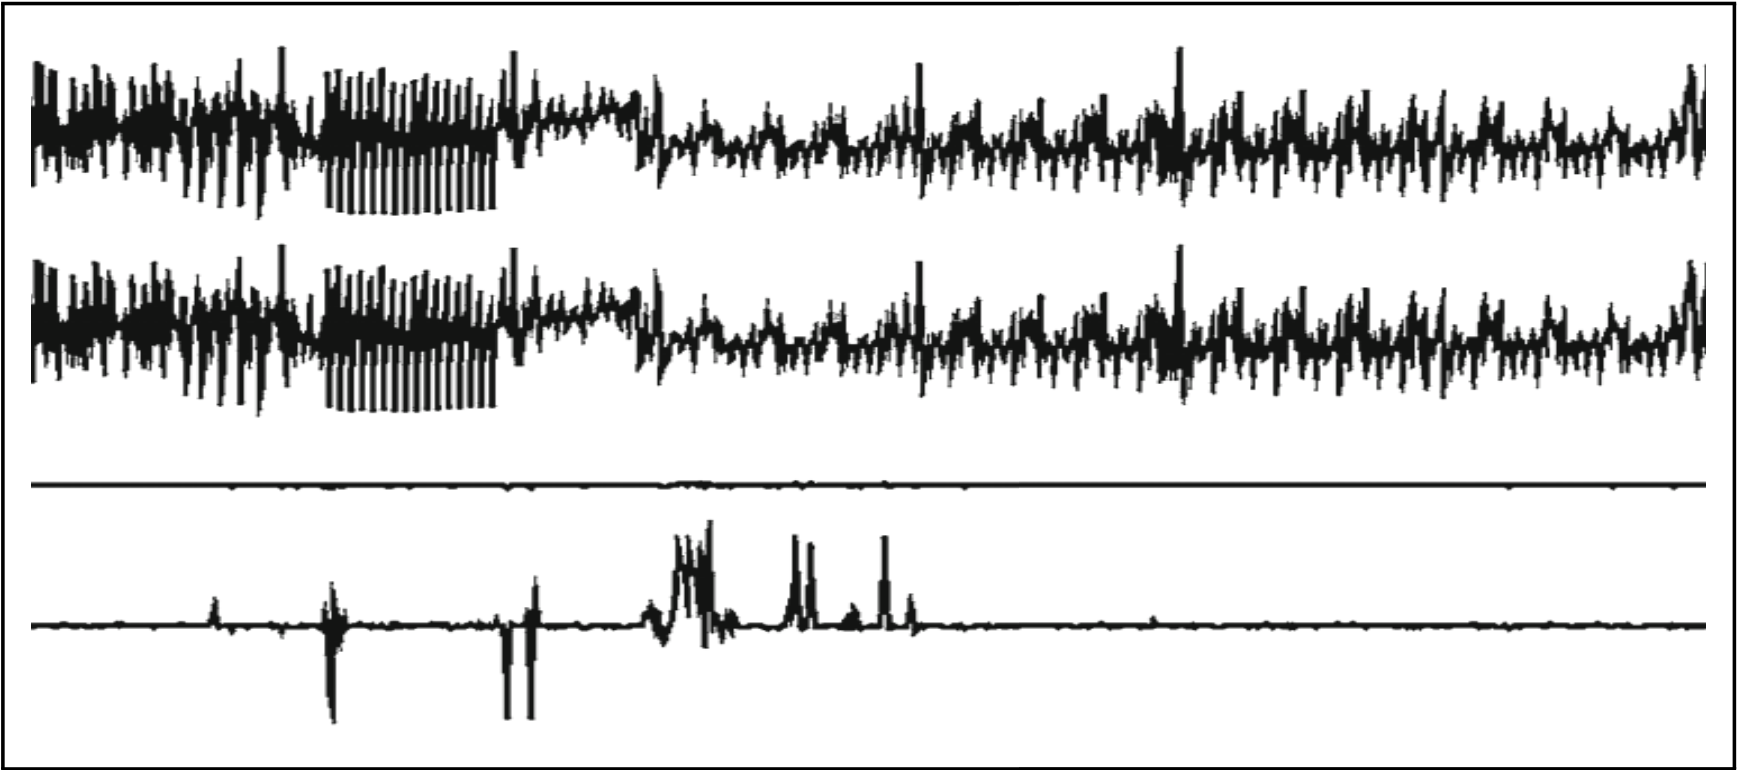
\includegraphics[width=0.4\linewidth]{figures/chapter4/fig12-c.png}
  	\label{fig:4-12-c}
  }
  \quad\quad\quad
  \subfigure[密钥$k=101,\dots,105$时的差分]{
  	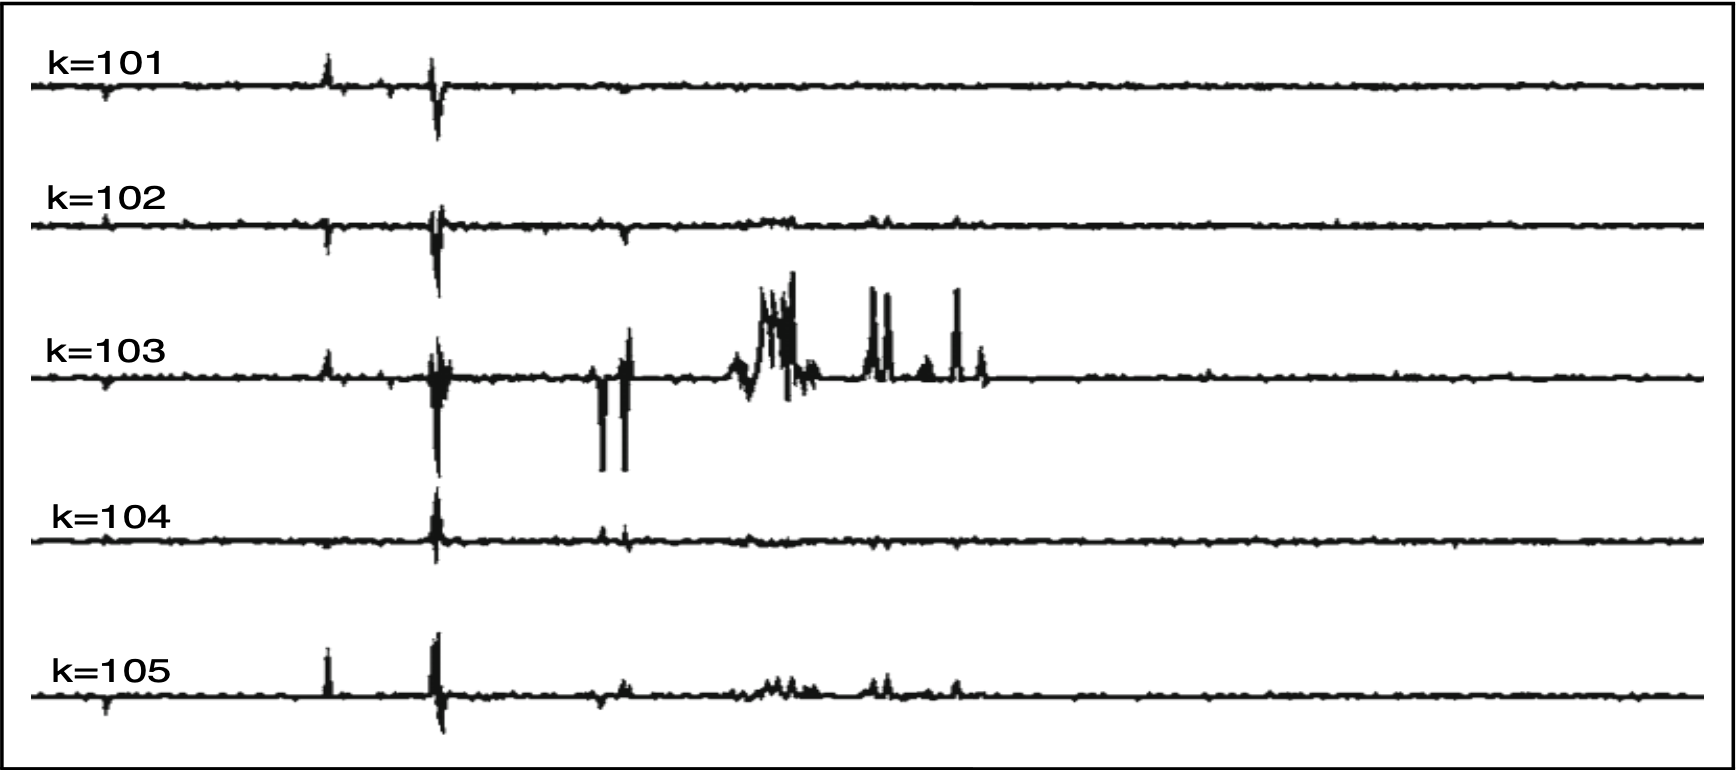
\includegraphics[width=0.4\linewidth]{figures/chapter4/fig12-d.png}
  	\label{fig:4-12-d}
  }
  \caption{针对AES的功耗分析}
\end{figure}

\begin{snote}[差分功耗分析。]
尽管 AES 对简单功耗攻击有抵抗能力,但一种更复杂的功耗攻击就能从一些简陋的 AES 算法实现中提取出 AES 密钥。随机选择一个 AES 密钥 $k$,并用它加密 $4000$ 条随机的明文。对于我们的测试设备来说,所产生的 $4000$ 个功耗轨迹图看起来非常不同,这表明在输入是随机明文的情况下,功耗轨迹与输入是相关的。

接下来,考虑第一轮中第一个 S 盒的输出,我们把这个输出称为 $T$。我们假设,S 盒查询的功耗取决于被查询的位置。也就是说,我们猜测 $T$ 的值与查表操作的功耗相关。

为了验证这个假设,我们根据 $T$ 的最小有效比特将 $4000$ 次的功率轨迹图分成两堆,第 $1$ 堆中 $T$ 的最小有效比特都为 $1$,第 $0$ 堆中 $T$ 的最小有效比特都为 $0$。考察加密信用卡在计算第一个 S 盒的输出时,每堆的功耗情况:
\begin{itemize}
	\item 第 $1$ 堆 (LSB $=1$):平均功耗 $116.9$ 个单位,标准差为 $10.7$
	\item 第 $0$ 堆 (LSB $=0$):平均功耗 $121.9$ 个单位,标准差为 $9.7$
\end{itemize}
图 \ref{fig:4-12-b} 展示了这两种功耗分布。这两个分布很接近,但有明显的不同。因此,只要有足够多的独立样本,我们就可以将两种分布区别开来。

为了利用这一观察,我们考察图 \ref{fig:4-12-c}。图中的第一行显示的是第 $1$ 堆中所有功耗轨迹的平均功耗情况。第二行显示的是第 $0$ 堆中所有功耗轨迹的平均功耗情况。最下面一行表示两条平均功耗轨迹的差分。我们可以发现,差分轨迹的第一个尖峰恰好位于计算第一个 S 盒输出时,而该尖峰的大小与图 \ref{fig:4-12-b} 中所显示的平均数之差完全对应。我们将这条差分轨迹称为\textbf{功耗差分 (power differential)}。

为了攻击目标设备,攻击者必须首先用一个干净的设备进行实验:攻击者将选定的密钥加载到设备中,并计算出设备的功耗差分轨迹,如图 \ref{fig:4-12-b} 所示。接下来,假设攻击者获得了一个带有未知的嵌入式密钥的设备,它就可以用以下方法提取密钥:
 
\vspace*{10pt}

\hspace*{5pt} 首先,对 $4000$ 条随机明文测量加密操作的功耗轨迹\\
\hspace*{26pt} 然后,对密钥首字节的每个候选值 $k\in\{0,1\}^8$,进行如下操作:\\
\hspace*{50pt} 根据 $T$ 的首个比特将 $4000$ 个样本分成两堆\\
\hspace*{75pt} (这是用目前对 $k$ 的猜测和 $4000$ 个已知的明文完成的)\\
\hspace*{50pt} 如果得到的功率差分轨迹与预先计算的曲线相匹配:\\
\hspace*{75pt} 输出 $k$ 作为密钥的首字节并停机

\vspace*{10pt}

\noindent
图 \ref{fig:4-12-d} 展示了这种攻击的效果。当使用密钥首字节的正确值(即 $k=103$)时,我们就能得到正确的功耗差分轨迹。而当使用错误的猜测($k=101,102,104,105$ 等)时,功耗差分与预期的轨迹不相符。

对 AES-128 密钥的所有 $16$ 个字节反复进行这一操作,就可以恢复整个密钥。
\end{snote}

\begin{snote}[缓和措施。]
针对功耗分析的一个常见的防御措施是进行硬件微调。从概念上讲,在执行 AES 之前,硬件会抽取固定数量的电力给电容器充电,然后利用电容器中的电力运行整个 AES 算法。一旦 AES 完成,留在电容器中的多余电量就会被丢弃。下一次应用 AES 时会再次给电容器充电,如此反复。这种概念设计(在实践中正确地实施需要一定程度的工作)旨在确保设备的功耗与设备中嵌入的密钥完全无关。

另一种缓和措施承认,每次运行解密算法都会泄露关于密钥的一些有限信息。这种措施提出在每次调用算法后重新随机化密钥,这样攻击者就不能将它从每次执行中获取到的信息结合起来。这种方法在一个被称为\textbf{抗泄露密码学 (leakage-resilient cryptography)}的领域中得到了广泛的研究。
\end{snote}

\subsection{针对AES的错误注入攻击}\label{subsec:4-3-3}

另一类攻击称为\textbf{错误注入攻击 (fault injection attack)},它试图故意在硬件运行密码系统时引入错误。攻击者可以利用畸形的输出来了解有关密钥的信息。注入错误可以通过对目标硬件进行超频,用激光加热,或对目标芯片进行电磁干扰来实现 \cite{joye2012fault}。

错误注入攻击已经被用来破解脆弱的 AES 实现,方法是迫使AES引擎在加密一个明文分组时发生故障。由此产生的畸变密文可以揭示有关密钥的信息 \cite{joye2012fault}。错误注入攻击也常被用在公钥密码场景中,我们将在 \ref{sec:17-6} 节回来详细地讨论它们,在那里,我们将介绍使用错误注入攻击完全破解 RSA 的一些实现的方法。

对错误注入攻击的一种防御措施是检查计算的结果。例如,AES 算法可以检查计算出的密文在解密后能否还原到给定的明文。如果检查失败,硬件就会抛出一个错误,并丢弃计算出的密文。但这种措施会将 AES 的性能降至原先的一半,因此不适合在实践中使用。

\subsection{量子穷举搜索攻击}\label{subsec:4-3-4}

到目前为止,我们描述的攻击都工作在经典计算机上。然而我们的物理世界是由量子力学定律所支配的。从理论上讲,人类可以构建基于量子力学定律的计算机,而这种计算机的计算能力要远超现在的经典计算机。尽管目前还没有人成功建造量子计算机,但第一台量子计算机的建成可能只是一个时间问题。

量子计算机对密码学有重大影响,因为它们可以被用来加速某些攻击,甚至完全打破一些系统。回顾一下,在经典的穷举搜索中,攻击者会得到一些用某个密钥 $k\in\mathcal{K}$ 创建的明文/密文对。攻击者会尝试所有的密钥,直到它找到一个能将给定的明文映射到给定的密文的密钥。在一台经典计算机上,这需要的时间与 $|\mathcal{K}|$ 成正比。


\begin{snote}[量子穷举搜索。]
令人惊讶的是,在量子计算机上,同样的穷举搜索的耗时只与 $\sqrt{|\mathcal{K}|}$ 成正比。这意味着对于像 AES-128 这样的分组密码,穷举搜索只需要大约 $\sqrt{2^{128}}=2^{64}$ 次计算。而使用经典计算机已经可以在合理的时间内完成 $2^{64}$ 步的计算,所以一旦量子计算机建成,它们也将能够进行这种规模的计算。因此,一旦量子计算机被制造出来,AES-128 将被认为是不安全的。

上述讨论表明,一个分组密码想要抵御量子穷举搜索攻击,其密钥空间 $|\mathcal{K}|$ 必须至少有 $2^{256}$ 那么大。此时,量子穷举搜索的时间是 $2^{128}$ 数量级的。量子计算机的这种威胁是 AES 支持 $256$ 比特密钥的原因之一。当然,我们不能保证没有更快的量子算法来破解 AES-256,但至少量子穷举搜索是不可能的。
\end{snote}

\begin{snote}[Grover 算法。]
量子穷举搜索算法是量子计算中一个更一般结论的特例,该结论由 Lov Grover 提出 \cite{grover1996fast}。该结论表明:假设我们有一个函数 $f:\mathcal{K}\to\{0,1\}$,对于某个 $k_0\in\mathcal{K}$,$f$ 的定义如下:
\begin{equation}\label{eq:4-20}
f(k)=\left\{
\begin{array}{ll}
1, & k=k_0\\
0, & k\neq k_0
\end{array}
\right.
\end{equation}
我们的目标是在只能``黑箱"访问 $f$(即只能在不同的输入情况下查询 $f$ 的输出)的情况下找到 $k_0$。在经典计算机上,没有任何其他方法的效率高于穷举所有的 $k\in\mathcal{K}$,在最糟糕的情况下,这需要对 $f$ 进行 $|\mathcal{K}|$ 数量级的查询。

Grover 算法表明,在量子计算机上只需 $O\big(\sqrt{|K|}\cdot{\rm time}(f)\big)$ 步就可以找到 $k_0$,其中 ${\rm time}(f)$ 表示计算 $f(x)$ 的耗时。这是个结论是普适的,它对任何形如式 \ref{eq:4-20} 的函数 $f$ 都成立。该结论可以用于加速一般的硬优化问题,是量子计算机的``杀手锏"。

在给定若干明文/密文对的情况下,为了破解一个像 AES-128 这样的分组密码,我们定义函数:
\[
f_{\rm AES}(k)=\left\{
\begin{array}{ll}
1, & {\rm AES}(k,\overline m)=\bar c\\
0, & \text{otherwise}
\end{array}
\right.
\]
其中 $\overline m=(m_0,\dots,m_Q)$,$\bar c=(c_0,\dots,c_Q)$ 是给定的明文和密文分组。假设给定足够多的分组,必定只有一个唯一的密钥 $k_0\in\mathcal{K}$ 满足 ${\rm AES}(k_0,\overline m)=\bar c$。而 Grover 算法可以在 $\sqrt{|\mathcal{K}|}$ 数量级的时间内找到这个密钥。
\end{snote}